% =====================================================================
%  reporte_2.tex
%  ========================
%
%
%  Descripción:
%  ------------
%  Reporte de la actividad 2 de Fundamentos para el Análisis Automático
%  de Lenguaje: pesado de los vectores con tf-idf y Okapi BM25,
%  recuperación por similitud coseno y evaluación contra los juicios
%  de relevancia de la colección Time.
%
%
%  Metadata:
%  ----------
%   * Author : zxxz6 (Bryan Violante Arriaga)
%   * Version: 1.0.0
%
%
%  History:
%  ------------
%  Author      Date            Description
%  zxxz6       14/09/2026      Creation
%
%
% =====================================================================
\documentclass[11pt,letterpaper]{article}

% =====================================================================
%  DATOS DE LA MATERIA
% =====================================================================
\newcommand{\materia}{Fundamentos para el Análisis Automático de Lenguaje}
\newcommand{\profesor}{Dra. Delia Irazú Hernández Farías \\
                       Dr. Luis Villaseñor Pineda \\
                       Dr. Manuel Montes y Gómez \\
                       Dr. Aurelio López López}
\newcommand{\periodo}{Otoño 2026}
\newcommand{\alumno}{Bryan Ezequiel Violante Arriaga}

% =====================================================================
%  Preambulo.tex
%  ========================
%
%
%  Descripción:
%  ------------
%  Preámbulo compartido de los apuntes de clase: paquetes, estilo de
%  página, entornos de teorema, las cuatro cajas de color, el estilo de
%  listings y el pseudocódigo en español. Se carga con \input desde
%  cada documento en lugar de copiarlo, para que un arreglo aquí llegue
%  a todas las libretas de una vez.
%
%
%  Considerations:
%  ------------
%  - Se carga con \input y ruta relativa, no con \usepackage, porque
%    \usepackage solo busca en la carpeta del documento y en el árbol
%    de TeX. Un .sty instalado en TEXMFHOME evitaría la ruta, pero vive
%    fuera del repo y una clona nueva no compilaría
%  - Los cuatro datos de la materia se declaran en el documento ANTES
%    del \input. hyperref expande \materia al cargarse, así que si no
%    existe todavía la compilación truena
%  - Cuando la materia la imparte más de un profesor, los nombres van
%    en un solo \profesor separados por \\. La portadilla los imprime
%    dentro de un center, que es donde \\ sí corta renglón. Repetir
%    \newcommand{\profesor} no es opción: truena con "already defined"
%  - algorithmicx no tiene opción de idioma y babel no lo traduce, así
%    que las palabras clave del pseudocódigo se renombran a mano
%  - Los nombres de los entornos van sin acento (\begin{definicion})
%    aunque el rótulo impreso sí lo lleve
%  - babel se carga con es-noshorthands porque en español el " queda
%    activo y se come el texto que le sigue, además de romper listings
%
%
%  Metadata:
%  ----------
%   * Author : zxxz6 (Bryan Violante Arriaga)
%   * Version: 1.7.0
%
%
%  History:
%  ------------
%  Author      Date            Description
%  zxxz6       24/09/2026      El nombre del alumno en el encabezado
%  zxxz6       24/09/2026      Encabezado de una hoja de un ejercicio
%  zxxz6       23/09/2026      Macros de los documentos de soluciones
%  zxxz6       30/08/2026      Macros de lim, limsup y liminf sobre n
%  zxxz6       25/08/2026      Macros de Omega, Theta, o y omega chicas
%  zxxz6       20/08/2026      Cargue pgfplots para graficas de datos
%  zxxz6       20/08/2026      Cargue tikz para diagramas de conjuntos
%  zxxz6       19/08/2026      Documente \profesor con varios nombres
%  zxxz6       19/08/2026      Agregue la caja Idea Random
%  zxxz6       18/08/2026      Creation
%
%
% =====================================================================
%  USO
%  ---
%  \documentclass[11pt,letterpaper]{article}
%  \newcommand{\materia}{...}      % los cuatro datos van arriba
%  \newcommand{\profesor}{...}
%  \newcommand{\periodo}{...}
%  \newcommand{\alumno}{...}
%  % =====================================================================
%  Preambulo.tex
%  ========================
%
%
%  Descripción:
%  ------------
%  Preámbulo compartido de los apuntes de clase: paquetes, estilo de
%  página, entornos de teorema, las cuatro cajas de color, el estilo de
%  listings y el pseudocódigo en español. Se carga con \input desde
%  cada documento en lugar de copiarlo, para que un arreglo aquí llegue
%  a todas las libretas de una vez.
%
%
%  Considerations:
%  ------------
%  - Se carga con \input y ruta relativa, no con \usepackage, porque
%    \usepackage solo busca en la carpeta del documento y en el árbol
%    de TeX. Un .sty instalado en TEXMFHOME evitaría la ruta, pero vive
%    fuera del repo y una clona nueva no compilaría
%  - Los cuatro datos de la materia se declaran en el documento ANTES
%    del \input. hyperref expande \materia al cargarse, así que si no
%    existe todavía la compilación truena
%  - Cuando la materia la imparte más de un profesor, los nombres van
%    en un solo \profesor separados por \\. La portadilla los imprime
%    dentro de un center, que es donde \\ sí corta renglón. Repetir
%    \newcommand{\profesor} no es opción: truena con "already defined"
%  - algorithmicx no tiene opción de idioma y babel no lo traduce, así
%    que las palabras clave del pseudocódigo se renombran a mano
%  - Los nombres de los entornos van sin acento (\begin{definicion})
%    aunque el rótulo impreso sí lo lleve
%  - babel se carga con es-noshorthands porque en español el " queda
%    activo y se come el texto que le sigue, además de romper listings
%
%
%  Metadata:
%  ----------
%   * Author : zxxz6 (Bryan Violante Arriaga)
%   * Version: 1.7.0
%
%
%  History:
%  ------------
%  Author      Date            Description
%  zxxz6       24/09/2026      El nombre del alumno en el encabezado
%  zxxz6       24/09/2026      Encabezado de una hoja de un ejercicio
%  zxxz6       23/09/2026      Macros de los documentos de soluciones
%  zxxz6       30/08/2026      Macros de lim, limsup y liminf sobre n
%  zxxz6       25/08/2026      Macros de Omega, Theta, o y omega chicas
%  zxxz6       20/08/2026      Cargue pgfplots para graficas de datos
%  zxxz6       20/08/2026      Cargue tikz para diagramas de conjuntos
%  zxxz6       19/08/2026      Documente \profesor con varios nombres
%  zxxz6       19/08/2026      Agregue la caja Idea Random
%  zxxz6       18/08/2026      Creation
%
%
% =====================================================================
%  USO
%  ---
%  \documentclass[11pt,letterpaper]{article}
%  \newcommand{\materia}{...}      % los cuatro datos van arriba
%  \newcommand{\profesor}{...}
%  \newcommand{\periodo}{...}
%  \newcommand{\alumno}{...}
%  % =====================================================================
%  Preambulo.tex
%  ========================
%
%
%  Descripción:
%  ------------
%  Preámbulo compartido de los apuntes de clase: paquetes, estilo de
%  página, entornos de teorema, las cuatro cajas de color, el estilo de
%  listings y el pseudocódigo en español. Se carga con \input desde
%  cada documento en lugar de copiarlo, para que un arreglo aquí llegue
%  a todas las libretas de una vez.
%
%
%  Considerations:
%  ------------
%  - Se carga con \input y ruta relativa, no con \usepackage, porque
%    \usepackage solo busca en la carpeta del documento y en el árbol
%    de TeX. Un .sty instalado en TEXMFHOME evitaría la ruta, pero vive
%    fuera del repo y una clona nueva no compilaría
%  - Los cuatro datos de la materia se declaran en el documento ANTES
%    del \input. hyperref expande \materia al cargarse, así que si no
%    existe todavía la compilación truena
%  - Cuando la materia la imparte más de un profesor, los nombres van
%    en un solo \profesor separados por \\. La portadilla los imprime
%    dentro de un center, que es donde \\ sí corta renglón. Repetir
%    \newcommand{\profesor} no es opción: truena con "already defined"
%  - algorithmicx no tiene opción de idioma y babel no lo traduce, así
%    que las palabras clave del pseudocódigo se renombran a mano
%  - Los nombres de los entornos van sin acento (\begin{definicion})
%    aunque el rótulo impreso sí lo lleve
%  - babel se carga con es-noshorthands porque en español el " queda
%    activo y se come el texto que le sigue, además de romper listings
%
%
%  Metadata:
%  ----------
%   * Author : zxxz6 (Bryan Violante Arriaga)
%   * Version: 1.7.0
%
%
%  History:
%  ------------
%  Author      Date            Description
%  zxxz6       24/09/2026      El nombre del alumno en el encabezado
%  zxxz6       24/09/2026      Encabezado de una hoja de un ejercicio
%  zxxz6       23/09/2026      Macros de los documentos de soluciones
%  zxxz6       30/08/2026      Macros de lim, limsup y liminf sobre n
%  zxxz6       25/08/2026      Macros de Omega, Theta, o y omega chicas
%  zxxz6       20/08/2026      Cargue pgfplots para graficas de datos
%  zxxz6       20/08/2026      Cargue tikz para diagramas de conjuntos
%  zxxz6       19/08/2026      Documente \profesor con varios nombres
%  zxxz6       19/08/2026      Agregue la caja Idea Random
%  zxxz6       18/08/2026      Creation
%
%
% =====================================================================
%  USO
%  ---
%  \documentclass[11pt,letterpaper]{article}
%  \newcommand{\materia}{...}      % los cuatro datos van arriba
%  \newcommand{\profesor}{...}
%  \newcommand{\periodo}{...}
%  \newcommand{\alumno}{...}
%  \input{../../templates/Preambulo.tex}
%  \begin{document}
%  \portadilla
%
%  Con dos o mas profesores se declara UN solo \profesor y los nombres
%  se separan con \\, uno por renglon:
%
%  \newcommand{\profesor}{Dra. Fulana de Tal \\
%                         Dr. Mengano de Cual}
% =====================================================================


% ==================== IDIOMA Y CODIFICACIÓN ====================
\usepackage[utf8]{inputenc}
\usepackage[T1]{fontenc}
\usepackage[spanish,es-tabla,es-noshorthands]{babel}
\usepackage{lmodern}
\usepackage{microtype}

% ==================== PÁGINA ====================
\usepackage[letterpaper,margin=2.3cm,headheight=14pt]{geometry}
\usepackage{parskip}
\usepackage{fancyhdr}
\usepackage{enumitem}

% ==================== MATEMÁTICAS ====================
\usepackage{amsmath,amssymb,amsthm,mathtools}

% ==================== FIGURAS, TABLAS, CÓDIGO ====================
\usepackage{graphicx}
\usepackage{booktabs}
\usepackage{array}
% float da el especificador [H], que clava una tabla donde se
% escribio. Una traza que LaTeX manda dos paginas adelante deja
% de leerse junto al paso que la produjo
\usepackage{float}
\usepackage{xcolor}
% tikz ya viene arrastrado por tcolorbox[most], pero se carga
% explicito para no depender de ese detalle; la libreria babel
% protege a tikz de los caracteres activos del español
\usepackage{tikz}
\usetikzlibrary{babel}
% pgfplots dibuja graficas de datos (ejes, escalas log) sobre tikz
\usepackage{pgfplots}
\pgfplotsset{compat=1.18}
\usepackage{listings}
\usepackage[ruled,section]{algorithm}
\usepackage{algpseudocode}
\usepackage[most]{tcolorbox}
% soul da \hl, el unico resaltado que parte renglon; \colorbox no
\usepackage{soul}
\usepackage{hyperref}

% =====================================================================
%  ESTILO
% =====================================================================

% --- encabezado y pie de cada página ---
\pagestyle{fancy}
\fancyhf{}
\fancyhead[L]{\small\textsc{\materia}}
\fancyhead[R]{\small\periodo}
\fancyfoot[C]{\small\thepage}
\renewcommand{\headrulewidth}{0.4pt}

% --- enlaces ---
\hypersetup{
  colorlinks=true,
  linkcolor=black,
  urlcolor=blue,
  citecolor=black,
  pdftitle={Apuntes de \materia},
  pdfauthor={\alumno}
}

% --- paleta ---
\definecolor{acento}{HTML}{1F4E79}
\definecolor{fondoIdea}{HTML}{EAF2FB}
\definecolor{fondoOjo}{HTML}{FDF0E6}
\definecolor{fondoPend}{HTML}{F2F0F7}
\definecolor{comentario}{HTML}{5A7D5A}
\definecolor{cadena}{HTML}{A03030}
\definecolor{fondoCodigo}{HTML}{F7F7F7}
\definecolor{fondoResultado}{HTML}{EAF5EC}
\definecolor{marcador}{HTML}{FFF3A3}

% --- entornos de teorema; numeran por sección, o sea por clase ---
\theoremstyle{definition}
\newtheorem{definicion}{Definición}[section]
\newtheorem{ejemplo}[definicion]{Ejemplo}
\newtheorem{ejercicio}[definicion]{Ejercicio}

\theoremstyle{plain}
\newtheorem{teorema}[definicion]{Teorema}
\newtheorem{lema}[definicion]{Lema}
\newtheorem{corolario}[definicion]{Corolario}
\newtheorem{proposicion}[definicion]{Proposición}

\theoremstyle{remark}
\newtheorem*{observacion}{Observación}
\newtheorem*{quick_sum}{Resumen rápido}

% --- cajas de color para lo que se relee antes del examen ---
\newtcolorbox{idea}[1][]{
  colback=fondoIdea, colframe=acento, boxrule=0.6pt,
  arc=2pt, left=6pt, right=6pt, top=5pt, bottom=5pt,
  title={Idea clave}, fonttitle=\bfseries\small, #1
}
\newtcolorbox{ojo}[1][]{
  colback=fondoOjo, colframe=orange!70!black, boxrule=0.6pt,
  arc=2pt, left=6pt, right=6pt, top=5pt, bottom=5pt,
  title={Ojito...}, fonttitle=\bfseries\small, #1
}
\newtcolorbox{pendiente}[1][]{
  colback=fondoPend, colframe=violet!60!black, boxrule=0.6pt,
  arc=2pt, left=6pt, right=6pt, top=5pt, bottom=5pt,
  title={Pendiente por resolver}, fonttitle=\bfseries\small, #1
}
\newtcolorbox{idear}[1][]{
  colback=fondoPend, colframe=pink!60!black, boxrule=0.6pt,
  arc=2pt, left=6pt, right=6pt, top=5pt, bottom=5pt,
  title={Idea Random}, fonttitle=\bfseries\small, #1
}

% --- el resultado al que llego un ejercicio, para que se vea de
%     lejos al hojear la hoja antes del examen ---
\newtcolorbox{resultado}[1][]{
  colback=fondoResultado, colframe=green!45!black, boxrule=0.6pt,
  arc=2pt, left=6pt, right=6pt, top=5pt, bottom=5pt,
  title={Resultado}, fonttitle=\bfseries\small, #1
}

% --- código ---
\lstdefinestyle{codigo}{
  backgroundcolor=\color{fondoCodigo},
  basicstyle=\ttfamily\footnotesize,
  keywordstyle=\color{acento}\bfseries,
  commentstyle=\color{comentario}\itshape,
  stringstyle=\color{cadena},
  numbers=left, numberstyle=\tiny\color{gray}, numbersep=8pt,
  frame=single, rulecolor=\color{gray!40},
  breaklines=true, showstringspaces=false,
  tabsize=4, captionpos=b,
  extendedchars=true, inputencoding=utf8,
  literate={á}{{\'a}}1 {é}{{\'e}}1 {í}{{\'i}}1
           {ó}{{\'o}}1 {ú}{{\'u}}1 {ñ}{{\~n}}1
           {Ü}{{\"U}}1 {ü}{{\"u}}1 {¿}{{?`}}1
           {¡}{{!`}}1
}
\lstset{style=codigo}
\renewcommand{\lstlistingname}{Código}
\renewcommand{\lstlistlistingname}{Índice de código}
% --- pseudocódigo; algorithmicx arma el cuerpo y algorithm el
%     flotante que lo numera y lo pone en el índice. Las palabras
%     clave vienen en inglés de fábrica y babel no las toca, así que
%     se renombran una por una ---
\floatname{algorithm}{Algoritmo}
\renewcommand{\listalgorithmname}{Índice de algoritmos}

\algrenewcommand\algorithmicrequire{\textbf{Entrada:}}
\algrenewcommand\algorithmicensure{\textbf{Salida:}}
\algrenewcommand\algorithmicend{\textbf{fin}}
\algrenewcommand\algorithmicif{\textbf{si}}
\algrenewcommand\algorithmicthen{\textbf{entonces}}
\algrenewcommand\algorithmicelse{\textbf{si no}}
\algrenewcommand\algorithmicfor{\textbf{para}}
\algrenewcommand\algorithmicforall{\textbf{para todo}}
\algrenewcommand\algorithmicdo{\textbf{hacer}}
\algrenewcommand\algorithmicwhile{\textbf{mientras}}
\algrenewcommand\algorithmicrepeat{\textbf{repetir}}
\algrenewcommand\algorithmicuntil{\textbf{hasta que}}
\algrenewcommand\algorithmicloop{\textbf{ciclo}}
\algrenewcommand\algorithmicprocedure{\textbf{procedimiento}}
\algrenewcommand\algorithmicfunction{\textbf{función}}
\algrenewcommand\algorithmicreturn{\textbf{devolver}}
\algrenewcomment[1]{\hfill{\color{comentario}\itshape // #1}}

% Las dos que algorithmicx no trae. El \ del final es obligatorio: sin
% el TeX se come el espacio y sale "hastan-1" en vez de "hasta n-1"
\algnewcommand\Hasta{\textbf{hasta}\ }
\algnewcommand\Intercambiar{\textbf{intercambiar}\ }

% --- abreviaturas que se usan a cada rato ---
\newcommand{\N}{\mathbb{N}}
\newcommand{\Z}{\mathbb{Z}}
\newcommand{\Q}{\mathbb{Q}}
\newcommand{\R}{\mathbb{R}}
\newcommand{\C}{\mathbb{C}}
\newcommand{\abs}[1]{\left\lvert #1 \right\rvert}
\newcommand{\norm}[1]{\left\lVert #1 \right\rVert}
\newcommand{\set}[1]{\left\{ #1 \right\}}
\newcommand{\Ord}[1]{\mathcal{O}\!\left(#1\right)}
% Mayuscula la notacion grande, minuscula la chica
\newcommand{\Omg}[1]{\Omega\!\left(#1\right)}
\newcommand{\Tht}[1]{\Theta\!\left(#1\right)}
\newcommand{\ord}[1]{o\!\left(#1\right)}
\newcommand{\omg}[1]{\omega\!\left(#1\right)}
% Los tres limites sobre n, que salen en cada renglon del criterio
% del cociente para la notacion asintotica
\newcommand{\LM}{\lim_{n \to \infty}}
\newcommand{\LS}{\limsup_{n \to \infty}}
\newcommand{\LI}{\liminf_{n \to \infty}}

% --- encabezado de cada sesión: título a la izquierda, fecha a la
%     derecha. El argumento corto es el que sale en el índice ---
\newcommand{\clase}[2]{%
  \section[#1]{#1 \hfill \normalfont\small\textit{#2}}%
}

% --- portadilla y tabla de contenidos. Se llama una vez, justo
%     despues de \begin{document}. El renglon del profesor va dentro
%     del center, asi que \profesor puede traer varios nombres
%     separados por \\ y salen apilados y centrados sin tocar nada ---
\newcommand{\portadilla}{%
  \begin{center}
    {\LARGE\bfseries\materia\par}
    \vspace{0.4em}
    {\large \profesor \par}
    \vspace{0.2em}
    {\small \periodo\quad-\quad\alumno\par}
    \vspace{0.3em}
    \rule{\linewidth}{0.5pt}
  \end{center}
  \vspace{0.5em}
  \tableofcontents
  \vspace{1em}
  \rule{\linewidth}{0.5pt}%
}

% =====================================================================
%  DOCUMENTOS DE SOLUCIONES
%  Lo que usa una tanda de ejercicios resueltos. Una libreta no toca
%  nada de aqui, pero vive en el preambulo compartido para no tener
%  dos archivos que arreglar cuando cambie el estilo.
% =====================================================================

% --- encabezado compacto: titulo, subtitulo y regla. Sustituye a
%     \portadilla cuando el documento es una tanda de ejercicios: sin
%     indice, porque se hojea de corrido, no se navega ---
\newcommand{\encabezadoSoluciones}[2]{%
  % El paquete algorithm se carga con la opcion [section] para que en
  % una libreta el pseudocodigo se numere por clase. Aqui no hay
  % secciones, asi que esa numeracion sale como "Algoritmo 0.1". Se
  % corrige al vuelo, y solo en los documentos que llaman a este
  % encabezado: la libreta no se entera.
  \renewcommand{\thealgorithm}{\arabic{algorithm}}%
  \begin{center}
    {\LARGE\bfseries #1\par}
    \vspace{0.3em}
    {\small\itshape #2\par}
    \vspace{0.5em}
    \rule{\linewidth}{0.5pt}
  \end{center}
  \vspace{0.3em}%
}

% --- hoja de un solo ejercicio: un renglon chico arriba con el
%     titulo y su numero, y ya. Sin titulo grande y sin pie de pagina,
%     porque en una hoja de dos paginas cada centimetro que se va en
%     adornos es un paso del desarrollo que no cabe ---
\newcommand{\encabezadoEjercicio}[3]{%
  % Misma correccion que en \encabezadoSoluciones: sin secciones, el
  % pseudocodigo saldria numerado "0.1"
  \renewcommand{\thealgorithm}{\arabic{algorithm}}%
  \fancyhf{}%
  \fancyhead[L]{\small\textsc{#1} (ejercicio #2 de #3)}%
  % El nombre va a la derecha porque las hojas de respuestas se
  % entregan y el profesor pide que cada una lo lleve
  \fancyhead[R]{\small\alumno}%
  \renewcommand{\headrulewidth}{0.4pt}%
  \pagestyle{fancy}%
  \thispagestyle{fancy}%
}

% --- bloque tematico, numerado con romanos: I, II, III. Agrupa los
%     ejercicios que comparten tema. No dibuja regla: la del
%     \problema que sigue ya separa el titulo del primer ejercicio,
%     y dos rayas seguidas dejan un hueco feo ---
\newcounter{parte}
\renewcommand{\theparte}{\Roman{parte}}
\newcommand{\parte}[1]{%
  \bigskip
  \refstepcounter{parte}%
  \noindent{\large\bfseries \theparte. #1\par}%
}

% --- un ejercicio resuelto. Se numera solo y corrido a lo largo del
%     documento, sin reiniciar en cada parte, para poder decir "el 14"
%     sin aclarar de que bloque ---
\newcounter{problema}
\newcommand{\problema}[1]{%
  \bigskip
  \noindent\rule{\linewidth}{0.4pt}\par
  \vspace{0.3em}
  \refstepcounter{problema}%
  \noindent{\bfseries Ejercicio \theproblema\ --- #1\par}
  \vspace{0.3em}%
}

% --- rotulo del paso que sigue: Caso base, Hipotesis inductiva, Paso
%     inductivo. El texto sigue en el mismo renglon ---
\newcommand{\paso}[1]{\par\vspace{0.3em}\noindent\textbf{#1}\ }

% --- la respuesta de un ejercicio, centrada y en un cuadro. El
%     argumento va en modo matematico, sin los delimitadores ---
\newcommand{\respuesta}[1]{%
  \[
    \boxed{\;#1\;}
  \]
}

% --- resaltado inline, como pasarle el plumon a media frase. No
%     admite matematicas adentro: soul rompe con $...$, asi que una
%     formula que hay que destacar va en \respuesta ---
\sethlcolor{marcador}
\newcommand{\resaltar}[1]{\hl{#1}}

% --- justificacion al final de un renglon de \align, en chiquito y
%     entre parentesis, para decir de donde salio el paso ---
\newcommand{\razon}[1]{\quad\text{\small\itshape (#1)}}

%############################ END OF PREAMBULO.TEX #############################
%###############################################################################

%  \begin{document}
%  \portadilla
%
%  Con dos o mas profesores se declara UN solo \profesor y los nombres
%  se separan con \\, uno por renglon:
%
%  \newcommand{\profesor}{Dra. Fulana de Tal \\
%                         Dr. Mengano de Cual}
% =====================================================================


% ==================== IDIOMA Y CODIFICACIÓN ====================
\usepackage[utf8]{inputenc}
\usepackage[T1]{fontenc}
\usepackage[spanish,es-tabla,es-noshorthands]{babel}
\usepackage{lmodern}
\usepackage{microtype}

% ==================== PÁGINA ====================
\usepackage[letterpaper,margin=2.3cm,headheight=14pt]{geometry}
\usepackage{parskip}
\usepackage{fancyhdr}
\usepackage{enumitem}

% ==================== MATEMÁTICAS ====================
\usepackage{amsmath,amssymb,amsthm,mathtools}

% ==================== FIGURAS, TABLAS, CÓDIGO ====================
\usepackage{graphicx}
\usepackage{booktabs}
\usepackage{array}
% float da el especificador [H], que clava una tabla donde se
% escribio. Una traza que LaTeX manda dos paginas adelante deja
% de leerse junto al paso que la produjo
\usepackage{float}
\usepackage{xcolor}
% tikz ya viene arrastrado por tcolorbox[most], pero se carga
% explicito para no depender de ese detalle; la libreria babel
% protege a tikz de los caracteres activos del español
\usepackage{tikz}
\usetikzlibrary{babel}
% pgfplots dibuja graficas de datos (ejes, escalas log) sobre tikz
\usepackage{pgfplots}
\pgfplotsset{compat=1.18}
\usepackage{listings}
\usepackage[ruled,section]{algorithm}
\usepackage{algpseudocode}
\usepackage[most]{tcolorbox}
% soul da \hl, el unico resaltado que parte renglon; \colorbox no
\usepackage{soul}
\usepackage{hyperref}

% =====================================================================
%  ESTILO
% =====================================================================

% --- encabezado y pie de cada página ---
\pagestyle{fancy}
\fancyhf{}
\fancyhead[L]{\small\textsc{\materia}}
\fancyhead[R]{\small\periodo}
\fancyfoot[C]{\small\thepage}
\renewcommand{\headrulewidth}{0.4pt}

% --- enlaces ---
\hypersetup{
  colorlinks=true,
  linkcolor=black,
  urlcolor=blue,
  citecolor=black,
  pdftitle={Apuntes de \materia},
  pdfauthor={\alumno}
}

% --- paleta ---
\definecolor{acento}{HTML}{1F4E79}
\definecolor{fondoIdea}{HTML}{EAF2FB}
\definecolor{fondoOjo}{HTML}{FDF0E6}
\definecolor{fondoPend}{HTML}{F2F0F7}
\definecolor{comentario}{HTML}{5A7D5A}
\definecolor{cadena}{HTML}{A03030}
\definecolor{fondoCodigo}{HTML}{F7F7F7}
\definecolor{fondoResultado}{HTML}{EAF5EC}
\definecolor{marcador}{HTML}{FFF3A3}

% --- entornos de teorema; numeran por sección, o sea por clase ---
\theoremstyle{definition}
\newtheorem{definicion}{Definición}[section]
\newtheorem{ejemplo}[definicion]{Ejemplo}
\newtheorem{ejercicio}[definicion]{Ejercicio}

\theoremstyle{plain}
\newtheorem{teorema}[definicion]{Teorema}
\newtheorem{lema}[definicion]{Lema}
\newtheorem{corolario}[definicion]{Corolario}
\newtheorem{proposicion}[definicion]{Proposición}

\theoremstyle{remark}
\newtheorem*{observacion}{Observación}
\newtheorem*{quick_sum}{Resumen rápido}

% --- cajas de color para lo que se relee antes del examen ---
\newtcolorbox{idea}[1][]{
  colback=fondoIdea, colframe=acento, boxrule=0.6pt,
  arc=2pt, left=6pt, right=6pt, top=5pt, bottom=5pt,
  title={Idea clave}, fonttitle=\bfseries\small, #1
}
\newtcolorbox{ojo}[1][]{
  colback=fondoOjo, colframe=orange!70!black, boxrule=0.6pt,
  arc=2pt, left=6pt, right=6pt, top=5pt, bottom=5pt,
  title={Ojito...}, fonttitle=\bfseries\small, #1
}
\newtcolorbox{pendiente}[1][]{
  colback=fondoPend, colframe=violet!60!black, boxrule=0.6pt,
  arc=2pt, left=6pt, right=6pt, top=5pt, bottom=5pt,
  title={Pendiente por resolver}, fonttitle=\bfseries\small, #1
}
\newtcolorbox{idear}[1][]{
  colback=fondoPend, colframe=pink!60!black, boxrule=0.6pt,
  arc=2pt, left=6pt, right=6pt, top=5pt, bottom=5pt,
  title={Idea Random}, fonttitle=\bfseries\small, #1
}

% --- el resultado al que llego un ejercicio, para que se vea de
%     lejos al hojear la hoja antes del examen ---
\newtcolorbox{resultado}[1][]{
  colback=fondoResultado, colframe=green!45!black, boxrule=0.6pt,
  arc=2pt, left=6pt, right=6pt, top=5pt, bottom=5pt,
  title={Resultado}, fonttitle=\bfseries\small, #1
}

% --- código ---
\lstdefinestyle{codigo}{
  backgroundcolor=\color{fondoCodigo},
  basicstyle=\ttfamily\footnotesize,
  keywordstyle=\color{acento}\bfseries,
  commentstyle=\color{comentario}\itshape,
  stringstyle=\color{cadena},
  numbers=left, numberstyle=\tiny\color{gray}, numbersep=8pt,
  frame=single, rulecolor=\color{gray!40},
  breaklines=true, showstringspaces=false,
  tabsize=4, captionpos=b,
  extendedchars=true, inputencoding=utf8,
  literate={á}{{\'a}}1 {é}{{\'e}}1 {í}{{\'i}}1
           {ó}{{\'o}}1 {ú}{{\'u}}1 {ñ}{{\~n}}1
           {Ü}{{\"U}}1 {ü}{{\"u}}1 {¿}{{?`}}1
           {¡}{{!`}}1
}
\lstset{style=codigo}
\renewcommand{\lstlistingname}{Código}
\renewcommand{\lstlistlistingname}{Índice de código}
% --- pseudocódigo; algorithmicx arma el cuerpo y algorithm el
%     flotante que lo numera y lo pone en el índice. Las palabras
%     clave vienen en inglés de fábrica y babel no las toca, así que
%     se renombran una por una ---
\floatname{algorithm}{Algoritmo}
\renewcommand{\listalgorithmname}{Índice de algoritmos}

\algrenewcommand\algorithmicrequire{\textbf{Entrada:}}
\algrenewcommand\algorithmicensure{\textbf{Salida:}}
\algrenewcommand\algorithmicend{\textbf{fin}}
\algrenewcommand\algorithmicif{\textbf{si}}
\algrenewcommand\algorithmicthen{\textbf{entonces}}
\algrenewcommand\algorithmicelse{\textbf{si no}}
\algrenewcommand\algorithmicfor{\textbf{para}}
\algrenewcommand\algorithmicforall{\textbf{para todo}}
\algrenewcommand\algorithmicdo{\textbf{hacer}}
\algrenewcommand\algorithmicwhile{\textbf{mientras}}
\algrenewcommand\algorithmicrepeat{\textbf{repetir}}
\algrenewcommand\algorithmicuntil{\textbf{hasta que}}
\algrenewcommand\algorithmicloop{\textbf{ciclo}}
\algrenewcommand\algorithmicprocedure{\textbf{procedimiento}}
\algrenewcommand\algorithmicfunction{\textbf{función}}
\algrenewcommand\algorithmicreturn{\textbf{devolver}}
\algrenewcomment[1]{\hfill{\color{comentario}\itshape // #1}}

% Las dos que algorithmicx no trae. El \ del final es obligatorio: sin
% el TeX se come el espacio y sale "hastan-1" en vez de "hasta n-1"
\algnewcommand\Hasta{\textbf{hasta}\ }
\algnewcommand\Intercambiar{\textbf{intercambiar}\ }

% --- abreviaturas que se usan a cada rato ---
\newcommand{\N}{\mathbb{N}}
\newcommand{\Z}{\mathbb{Z}}
\newcommand{\Q}{\mathbb{Q}}
\newcommand{\R}{\mathbb{R}}
\newcommand{\C}{\mathbb{C}}
\newcommand{\abs}[1]{\left\lvert #1 \right\rvert}
\newcommand{\norm}[1]{\left\lVert #1 \right\rVert}
\newcommand{\set}[1]{\left\{ #1 \right\}}
\newcommand{\Ord}[1]{\mathcal{O}\!\left(#1\right)}
% Mayuscula la notacion grande, minuscula la chica
\newcommand{\Omg}[1]{\Omega\!\left(#1\right)}
\newcommand{\Tht}[1]{\Theta\!\left(#1\right)}
\newcommand{\ord}[1]{o\!\left(#1\right)}
\newcommand{\omg}[1]{\omega\!\left(#1\right)}
% Los tres limites sobre n, que salen en cada renglon del criterio
% del cociente para la notacion asintotica
\newcommand{\LM}{\lim_{n \to \infty}}
\newcommand{\LS}{\limsup_{n \to \infty}}
\newcommand{\LI}{\liminf_{n \to \infty}}

% --- encabezado de cada sesión: título a la izquierda, fecha a la
%     derecha. El argumento corto es el que sale en el índice ---
\newcommand{\clase}[2]{%
  \section[#1]{#1 \hfill \normalfont\small\textit{#2}}%
}

% --- portadilla y tabla de contenidos. Se llama una vez, justo
%     despues de \begin{document}. El renglon del profesor va dentro
%     del center, asi que \profesor puede traer varios nombres
%     separados por \\ y salen apilados y centrados sin tocar nada ---
\newcommand{\portadilla}{%
  \begin{center}
    {\LARGE\bfseries\materia\par}
    \vspace{0.4em}
    {\large \profesor \par}
    \vspace{0.2em}
    {\small \periodo\quad-\quad\alumno\par}
    \vspace{0.3em}
    \rule{\linewidth}{0.5pt}
  \end{center}
  \vspace{0.5em}
  \tableofcontents
  \vspace{1em}
  \rule{\linewidth}{0.5pt}%
}

% =====================================================================
%  DOCUMENTOS DE SOLUCIONES
%  Lo que usa una tanda de ejercicios resueltos. Una libreta no toca
%  nada de aqui, pero vive en el preambulo compartido para no tener
%  dos archivos que arreglar cuando cambie el estilo.
% =====================================================================

% --- encabezado compacto: titulo, subtitulo y regla. Sustituye a
%     \portadilla cuando el documento es una tanda de ejercicios: sin
%     indice, porque se hojea de corrido, no se navega ---
\newcommand{\encabezadoSoluciones}[2]{%
  % El paquete algorithm se carga con la opcion [section] para que en
  % una libreta el pseudocodigo se numere por clase. Aqui no hay
  % secciones, asi que esa numeracion sale como "Algoritmo 0.1". Se
  % corrige al vuelo, y solo en los documentos que llaman a este
  % encabezado: la libreta no se entera.
  \renewcommand{\thealgorithm}{\arabic{algorithm}}%
  \begin{center}
    {\LARGE\bfseries #1\par}
    \vspace{0.3em}
    {\small\itshape #2\par}
    \vspace{0.5em}
    \rule{\linewidth}{0.5pt}
  \end{center}
  \vspace{0.3em}%
}

% --- hoja de un solo ejercicio: un renglon chico arriba con el
%     titulo y su numero, y ya. Sin titulo grande y sin pie de pagina,
%     porque en una hoja de dos paginas cada centimetro que se va en
%     adornos es un paso del desarrollo que no cabe ---
\newcommand{\encabezadoEjercicio}[3]{%
  % Misma correccion que en \encabezadoSoluciones: sin secciones, el
  % pseudocodigo saldria numerado "0.1"
  \renewcommand{\thealgorithm}{\arabic{algorithm}}%
  \fancyhf{}%
  \fancyhead[L]{\small\textsc{#1} (ejercicio #2 de #3)}%
  % El nombre va a la derecha porque las hojas de respuestas se
  % entregan y el profesor pide que cada una lo lleve
  \fancyhead[R]{\small\alumno}%
  \renewcommand{\headrulewidth}{0.4pt}%
  \pagestyle{fancy}%
  \thispagestyle{fancy}%
}

% --- bloque tematico, numerado con romanos: I, II, III. Agrupa los
%     ejercicios que comparten tema. No dibuja regla: la del
%     \problema que sigue ya separa el titulo del primer ejercicio,
%     y dos rayas seguidas dejan un hueco feo ---
\newcounter{parte}
\renewcommand{\theparte}{\Roman{parte}}
\newcommand{\parte}[1]{%
  \bigskip
  \refstepcounter{parte}%
  \noindent{\large\bfseries \theparte. #1\par}%
}

% --- un ejercicio resuelto. Se numera solo y corrido a lo largo del
%     documento, sin reiniciar en cada parte, para poder decir "el 14"
%     sin aclarar de que bloque ---
\newcounter{problema}
\newcommand{\problema}[1]{%
  \bigskip
  \noindent\rule{\linewidth}{0.4pt}\par
  \vspace{0.3em}
  \refstepcounter{problema}%
  \noindent{\bfseries Ejercicio \theproblema\ --- #1\par}
  \vspace{0.3em}%
}

% --- rotulo del paso que sigue: Caso base, Hipotesis inductiva, Paso
%     inductivo. El texto sigue en el mismo renglon ---
\newcommand{\paso}[1]{\par\vspace{0.3em}\noindent\textbf{#1}\ }

% --- la respuesta de un ejercicio, centrada y en un cuadro. El
%     argumento va en modo matematico, sin los delimitadores ---
\newcommand{\respuesta}[1]{%
  \[
    \boxed{\;#1\;}
  \]
}

% --- resaltado inline, como pasarle el plumon a media frase. No
%     admite matematicas adentro: soul rompe con $...$, asi que una
%     formula que hay que destacar va en \respuesta ---
\sethlcolor{marcador}
\newcommand{\resaltar}[1]{\hl{#1}}

% --- justificacion al final de un renglon de \align, en chiquito y
%     entre parentesis, para decir de donde salio el paso ---
\newcommand{\razon}[1]{\quad\text{\small\itshape (#1)}}

%############################ END OF PREAMBULO.TEX #############################
%###############################################################################

%  \begin{document}
%  \portadilla
%
%  Con dos o mas profesores se declara UN solo \profesor y los nombres
%  se separan con \\, uno por renglon:
%
%  \newcommand{\profesor}{Dra. Fulana de Tal \\
%                         Dr. Mengano de Cual}
% =====================================================================


% ==================== IDIOMA Y CODIFICACIÓN ====================
\usepackage[utf8]{inputenc}
\usepackage[T1]{fontenc}
\usepackage[spanish,es-tabla,es-noshorthands]{babel}
\usepackage{lmodern}
\usepackage{microtype}

% ==================== PÁGINA ====================
\usepackage[letterpaper,margin=2.3cm,headheight=14pt]{geometry}
\usepackage{parskip}
\usepackage{fancyhdr}
\usepackage{enumitem}

% ==================== MATEMÁTICAS ====================
\usepackage{amsmath,amssymb,amsthm,mathtools}

% ==================== FIGURAS, TABLAS, CÓDIGO ====================
\usepackage{graphicx}
\usepackage{booktabs}
\usepackage{array}
% float da el especificador [H], que clava una tabla donde se
% escribio. Una traza que LaTeX manda dos paginas adelante deja
% de leerse junto al paso que la produjo
\usepackage{float}
\usepackage{xcolor}
% tikz ya viene arrastrado por tcolorbox[most], pero se carga
% explicito para no depender de ese detalle; la libreria babel
% protege a tikz de los caracteres activos del español
\usepackage{tikz}
\usetikzlibrary{babel}
% pgfplots dibuja graficas de datos (ejes, escalas log) sobre tikz
\usepackage{pgfplots}
\pgfplotsset{compat=1.18}
\usepackage{listings}
\usepackage[ruled,section]{algorithm}
\usepackage{algpseudocode}
\usepackage[most]{tcolorbox}
% soul da \hl, el unico resaltado que parte renglon; \colorbox no
\usepackage{soul}
\usepackage{hyperref}

% =====================================================================
%  ESTILO
% =====================================================================

% --- encabezado y pie de cada página ---
\pagestyle{fancy}
\fancyhf{}
\fancyhead[L]{\small\textsc{\materia}}
\fancyhead[R]{\small\periodo}
\fancyfoot[C]{\small\thepage}
\renewcommand{\headrulewidth}{0.4pt}

% --- enlaces ---
\hypersetup{
  colorlinks=true,
  linkcolor=black,
  urlcolor=blue,
  citecolor=black,
  pdftitle={Apuntes de \materia},
  pdfauthor={\alumno}
}

% --- paleta ---
\definecolor{acento}{HTML}{1F4E79}
\definecolor{fondoIdea}{HTML}{EAF2FB}
\definecolor{fondoOjo}{HTML}{FDF0E6}
\definecolor{fondoPend}{HTML}{F2F0F7}
\definecolor{comentario}{HTML}{5A7D5A}
\definecolor{cadena}{HTML}{A03030}
\definecolor{fondoCodigo}{HTML}{F7F7F7}
\definecolor{fondoResultado}{HTML}{EAF5EC}
\definecolor{marcador}{HTML}{FFF3A3}

% --- entornos de teorema; numeran por sección, o sea por clase ---
\theoremstyle{definition}
\newtheorem{definicion}{Definición}[section]
\newtheorem{ejemplo}[definicion]{Ejemplo}
\newtheorem{ejercicio}[definicion]{Ejercicio}

\theoremstyle{plain}
\newtheorem{teorema}[definicion]{Teorema}
\newtheorem{lema}[definicion]{Lema}
\newtheorem{corolario}[definicion]{Corolario}
\newtheorem{proposicion}[definicion]{Proposición}

\theoremstyle{remark}
\newtheorem*{observacion}{Observación}
\newtheorem*{quick_sum}{Resumen rápido}

% --- cajas de color para lo que se relee antes del examen ---
\newtcolorbox{idea}[1][]{
  colback=fondoIdea, colframe=acento, boxrule=0.6pt,
  arc=2pt, left=6pt, right=6pt, top=5pt, bottom=5pt,
  title={Idea clave}, fonttitle=\bfseries\small, #1
}
\newtcolorbox{ojo}[1][]{
  colback=fondoOjo, colframe=orange!70!black, boxrule=0.6pt,
  arc=2pt, left=6pt, right=6pt, top=5pt, bottom=5pt,
  title={Ojito...}, fonttitle=\bfseries\small, #1
}
\newtcolorbox{pendiente}[1][]{
  colback=fondoPend, colframe=violet!60!black, boxrule=0.6pt,
  arc=2pt, left=6pt, right=6pt, top=5pt, bottom=5pt,
  title={Pendiente por resolver}, fonttitle=\bfseries\small, #1
}
\newtcolorbox{idear}[1][]{
  colback=fondoPend, colframe=pink!60!black, boxrule=0.6pt,
  arc=2pt, left=6pt, right=6pt, top=5pt, bottom=5pt,
  title={Idea Random}, fonttitle=\bfseries\small, #1
}

% --- el resultado al que llego un ejercicio, para que se vea de
%     lejos al hojear la hoja antes del examen ---
\newtcolorbox{resultado}[1][]{
  colback=fondoResultado, colframe=green!45!black, boxrule=0.6pt,
  arc=2pt, left=6pt, right=6pt, top=5pt, bottom=5pt,
  title={Resultado}, fonttitle=\bfseries\small, #1
}

% --- código ---
\lstdefinestyle{codigo}{
  backgroundcolor=\color{fondoCodigo},
  basicstyle=\ttfamily\footnotesize,
  keywordstyle=\color{acento}\bfseries,
  commentstyle=\color{comentario}\itshape,
  stringstyle=\color{cadena},
  numbers=left, numberstyle=\tiny\color{gray}, numbersep=8pt,
  frame=single, rulecolor=\color{gray!40},
  breaklines=true, showstringspaces=false,
  tabsize=4, captionpos=b,
  extendedchars=true, inputencoding=utf8,
  literate={á}{{\'a}}1 {é}{{\'e}}1 {í}{{\'i}}1
           {ó}{{\'o}}1 {ú}{{\'u}}1 {ñ}{{\~n}}1
           {Ü}{{\"U}}1 {ü}{{\"u}}1 {¿}{{?`}}1
           {¡}{{!`}}1
}
\lstset{style=codigo}
\renewcommand{\lstlistingname}{Código}
\renewcommand{\lstlistlistingname}{Índice de código}
% --- pseudocódigo; algorithmicx arma el cuerpo y algorithm el
%     flotante que lo numera y lo pone en el índice. Las palabras
%     clave vienen en inglés de fábrica y babel no las toca, así que
%     se renombran una por una ---
\floatname{algorithm}{Algoritmo}
\renewcommand{\listalgorithmname}{Índice de algoritmos}

\algrenewcommand\algorithmicrequire{\textbf{Entrada:}}
\algrenewcommand\algorithmicensure{\textbf{Salida:}}
\algrenewcommand\algorithmicend{\textbf{fin}}
\algrenewcommand\algorithmicif{\textbf{si}}
\algrenewcommand\algorithmicthen{\textbf{entonces}}
\algrenewcommand\algorithmicelse{\textbf{si no}}
\algrenewcommand\algorithmicfor{\textbf{para}}
\algrenewcommand\algorithmicforall{\textbf{para todo}}
\algrenewcommand\algorithmicdo{\textbf{hacer}}
\algrenewcommand\algorithmicwhile{\textbf{mientras}}
\algrenewcommand\algorithmicrepeat{\textbf{repetir}}
\algrenewcommand\algorithmicuntil{\textbf{hasta que}}
\algrenewcommand\algorithmicloop{\textbf{ciclo}}
\algrenewcommand\algorithmicprocedure{\textbf{procedimiento}}
\algrenewcommand\algorithmicfunction{\textbf{función}}
\algrenewcommand\algorithmicreturn{\textbf{devolver}}
\algrenewcomment[1]{\hfill{\color{comentario}\itshape // #1}}

% Las dos que algorithmicx no trae. El \ del final es obligatorio: sin
% el TeX se come el espacio y sale "hastan-1" en vez de "hasta n-1"
\algnewcommand\Hasta{\textbf{hasta}\ }
\algnewcommand\Intercambiar{\textbf{intercambiar}\ }

% --- abreviaturas que se usan a cada rato ---
\newcommand{\N}{\mathbb{N}}
\newcommand{\Z}{\mathbb{Z}}
\newcommand{\Q}{\mathbb{Q}}
\newcommand{\R}{\mathbb{R}}
\newcommand{\C}{\mathbb{C}}
\newcommand{\abs}[1]{\left\lvert #1 \right\rvert}
\newcommand{\norm}[1]{\left\lVert #1 \right\rVert}
\newcommand{\set}[1]{\left\{ #1 \right\}}
\newcommand{\Ord}[1]{\mathcal{O}\!\left(#1\right)}
% Mayuscula la notacion grande, minuscula la chica
\newcommand{\Omg}[1]{\Omega\!\left(#1\right)}
\newcommand{\Tht}[1]{\Theta\!\left(#1\right)}
\newcommand{\ord}[1]{o\!\left(#1\right)}
\newcommand{\omg}[1]{\omega\!\left(#1\right)}
% Los tres limites sobre n, que salen en cada renglon del criterio
% del cociente para la notacion asintotica
\newcommand{\LM}{\lim_{n \to \infty}}
\newcommand{\LS}{\limsup_{n \to \infty}}
\newcommand{\LI}{\liminf_{n \to \infty}}

% --- encabezado de cada sesión: título a la izquierda, fecha a la
%     derecha. El argumento corto es el que sale en el índice ---
\newcommand{\clase}[2]{%
  \section[#1]{#1 \hfill \normalfont\small\textit{#2}}%
}

% --- portadilla y tabla de contenidos. Se llama una vez, justo
%     despues de \begin{document}. El renglon del profesor va dentro
%     del center, asi que \profesor puede traer varios nombres
%     separados por \\ y salen apilados y centrados sin tocar nada ---
\newcommand{\portadilla}{%
  \begin{center}
    {\LARGE\bfseries\materia\par}
    \vspace{0.4em}
    {\large \profesor \par}
    \vspace{0.2em}
    {\small \periodo\quad-\quad\alumno\par}
    \vspace{0.3em}
    \rule{\linewidth}{0.5pt}
  \end{center}
  \vspace{0.5em}
  \tableofcontents
  \vspace{1em}
  \rule{\linewidth}{0.5pt}%
}

% =====================================================================
%  DOCUMENTOS DE SOLUCIONES
%  Lo que usa una tanda de ejercicios resueltos. Una libreta no toca
%  nada de aqui, pero vive en el preambulo compartido para no tener
%  dos archivos que arreglar cuando cambie el estilo.
% =====================================================================

% --- encabezado compacto: titulo, subtitulo y regla. Sustituye a
%     \portadilla cuando el documento es una tanda de ejercicios: sin
%     indice, porque se hojea de corrido, no se navega ---
\newcommand{\encabezadoSoluciones}[2]{%
  % El paquete algorithm se carga con la opcion [section] para que en
  % una libreta el pseudocodigo se numere por clase. Aqui no hay
  % secciones, asi que esa numeracion sale como "Algoritmo 0.1". Se
  % corrige al vuelo, y solo en los documentos que llaman a este
  % encabezado: la libreta no se entera.
  \renewcommand{\thealgorithm}{\arabic{algorithm}}%
  \begin{center}
    {\LARGE\bfseries #1\par}
    \vspace{0.3em}
    {\small\itshape #2\par}
    \vspace{0.5em}
    \rule{\linewidth}{0.5pt}
  \end{center}
  \vspace{0.3em}%
}

% --- hoja de un solo ejercicio: un renglon chico arriba con el
%     titulo y su numero, y ya. Sin titulo grande y sin pie de pagina,
%     porque en una hoja de dos paginas cada centimetro que se va en
%     adornos es un paso del desarrollo que no cabe ---
\newcommand{\encabezadoEjercicio}[3]{%
  % Misma correccion que en \encabezadoSoluciones: sin secciones, el
  % pseudocodigo saldria numerado "0.1"
  \renewcommand{\thealgorithm}{\arabic{algorithm}}%
  \fancyhf{}%
  \fancyhead[L]{\small\textsc{#1} (ejercicio #2 de #3)}%
  % El nombre va a la derecha porque las hojas de respuestas se
  % entregan y el profesor pide que cada una lo lleve
  \fancyhead[R]{\small\alumno}%
  \renewcommand{\headrulewidth}{0.4pt}%
  \pagestyle{fancy}%
  \thispagestyle{fancy}%
}

% --- bloque tematico, numerado con romanos: I, II, III. Agrupa los
%     ejercicios que comparten tema. No dibuja regla: la del
%     \problema que sigue ya separa el titulo del primer ejercicio,
%     y dos rayas seguidas dejan un hueco feo ---
\newcounter{parte}
\renewcommand{\theparte}{\Roman{parte}}
\newcommand{\parte}[1]{%
  \bigskip
  \refstepcounter{parte}%
  \noindent{\large\bfseries \theparte. #1\par}%
}

% --- un ejercicio resuelto. Se numera solo y corrido a lo largo del
%     documento, sin reiniciar en cada parte, para poder decir "el 14"
%     sin aclarar de que bloque ---
\newcounter{problema}
\newcommand{\problema}[1]{%
  \bigskip
  \noindent\rule{\linewidth}{0.4pt}\par
  \vspace{0.3em}
  \refstepcounter{problema}%
  \noindent{\bfseries Ejercicio \theproblema\ --- #1\par}
  \vspace{0.3em}%
}

% --- rotulo del paso que sigue: Caso base, Hipotesis inductiva, Paso
%     inductivo. El texto sigue en el mismo renglon ---
\newcommand{\paso}[1]{\par\vspace{0.3em}\noindent\textbf{#1}\ }

% --- la respuesta de un ejercicio, centrada y en un cuadro. El
%     argumento va en modo matematico, sin los delimitadores ---
\newcommand{\respuesta}[1]{%
  \[
    \boxed{\;#1\;}
  \]
}

% --- resaltado inline, como pasarle el plumon a media frase. No
%     admite matematicas adentro: soul rompe con $...$, asi que una
%     formula que hay que destacar va en \respuesta ---
\sethlcolor{marcador}
\newcommand{\resaltar}[1]{\hl{#1}}

% --- justificacion al final de un renglon de \align, en chiquito y
%     entre parentesis, para decir de donde salio el paso ---
\newcommand{\razon}[1]{\quad\text{\small\itshape (#1)}}

%############################ END OF PREAMBULO.TEX #############################
%###############################################################################


% El preambulo compartido pone el numero de pagina en el pie. Un
% reporte de cuatro hojas no lo necesita, asi que se limpia solo aqui.
\fancyfoot[C]{}

% =====================================================================
\begin{document}
% =====================================================================

\begin{center}
  {\LARGE\bfseries Actividad 2\par}
  \vspace{0.3em}
  {\large Pesado, recuperación y evaluación sobre la colección
   Time\par}
  \vspace{0.5em}
  {\small \alumno \quad-\quad \periodo\par}
  \vspace{0.4em}
  \rule{\linewidth}{0.5pt}
\end{center}

\section*{Resumen}

Partiendo del vocabulario obtenido en la actividad 1, se construyeron
los vectores de los 423 documentos con pesado tf-idf y los de las 83
consultas con pesado binario, y se recuperó por similitud coseno para
las primeras 10 consultas. Se evaluó contra los juicios de relevancia
de la colección calculando precisión, recuerdo y $F_1$. Como
comparación adicional se repitió todo con Okapi BM25 y sobre los dos
corpus truncados disponibles, el de Porter original y el de NLTK, lo
que da cuatro sistemas.

\section{Punto de partida}

De la actividad 1 se heredan las matrices documento-término con las
frecuencias crudas, para los dos modos de truncamiento.

\begin{center}
\begin{tabular}{lrrr}
    \toprule
    \textbf{Corpus} & \textbf{Documentos} & \textbf{Términos}
      & \textbf{Celdas no nulas} \\
    \midrule
    Porter (1980) & 423 & 16\,675 & 92\,091 \\
    Porter (NLTK) & 423 & 16\,623 & 92\,040 \\
    \bottomrule
\end{tabular}
\end{center}

Las consultas se procesaron con el mismo pipeline y se realinearon al
vocabulario de los documentos, de modo que ambos lados viven en el
mismo espacio. Tienen entre 3 y 18 términos, con $8.7$ de promedio.

\section{Método}

\subsection*{Pesado de los documentos}

El pesado tf-idf sigue la definición que vimos en clase. La frecuencia se
normaliza contra el término más frecuente del documento y se multiplica
por el idf con logaritmo natural:
\[
    w_{i,j} = \frac{f_{i,j}}{\max_k f_{k,j}}
              \cdot \log \frac{N}{n_i} ,
\]
con $N = 423$ y $n_i$ el número de documentos que contienen al término
$i$. La base del logaritmo solo escala todo por igual y no altera el
orden del ranking.

Okapi BM25 se incluyó como comparación. Satura la frecuencia y
normaliza contra la longitud promedio de la colección en vez de contra
el pico del propio documento:
\[
    w_{i,j} = \log\!\left(\frac{N - n_i + 0.5}{n_i + 0.5} + 1\right)
              \cdot
              \frac{f_{i,j}\,(k_1 + 1)}
                   {f_{i,j} + k_1\left(1 - b
                    + b\,\frac{|d_j|}{\overline{|d|}}\right)} ,
\]
con los valores clásicos $k_1 = 1.2$ y $b = 0.75$. El $+1$ dentro del
logaritmo mantiene el idf no negativo; sin él, un término presente en
más de la mitad de la colección tendría peso negativo y restaría.



\subsection*{Pesado de las consultas y recuperación}

Las consultas llevan pesado binario (usar $tf$ seria igual que binario), 
todo término presente vale $1$ y todo faltante vale $0$.

La IR es por similitud coseno, normalizando ambos lados
antes de multiplicar:
\[
    \mathrm{sim}(d, q) = \frac{d \cdot q}{\|d\|\,\|q\|} .
\]
Se conservan los documentos de coseno distinto de cero y se ordenan de
forma decreciente


\subsection*{Métricas de evaluación}

Sobre el ranking completo se calculan las tres medidas de conjunto
vistas en clase. Con $\mathrm{Rec}$ el conjunto recuperado y
$\mathrm{Rel}$ el de relevantes según los juicios:
\[
    P = \frac{|\mathrm{Rec} \cap \mathrm{Rel}|}{|\mathrm{Rec}|} ,
    \qquad
    R = \frac{|\mathrm{Rec} \cap \mathrm{Rel}|}{|\mathrm{Rel}|} ,
    \qquad
    F_1 = \frac{2 \cdot P \cdot R}{P + R} .
\]
El denominador de $R$ son todos los relevantes que existen, incluidos
los que el sistema nunca recuperó, así que castiga lo que se quedó
fuera. $F_1$ es la media armónica, que penaliza el desbalance: un
sistema con $P = 1$ y $R = 0.01$ promedia $0.5$ pero da
$F_1 = 0.02$.

Estas tres ignoran el orden, y por eso hizo falta agregar medidas
sensibles al rango, ya que todas salían iguales. 
La más simple es cortar el ranking en las primeras
$N$ posiciones y medir la precisión ahí:
\[
    P@N = \frac{\text{relevantes en las primeras } N}{N} .
\]
Se reportan $P@5$ y $P@10$.

La medida que resume el ranking entero es la precisión promedio, que
mide $P@k$ justo en cada posición donde apareció un relevante y
promedia esos valores. Su promedio sobre las consultas es el MAP:
\[
    \mathrm{AP}(q) = \frac{1}{|\mathrm{Rel}|} \sum_{k=1}^{n}
                     P@k \cdot \mathrm{rel}(k) ,
    \qquad
    \mathrm{MAP} = \frac{1}{|Q|} \sum_{q \in Q} \mathrm{AP}(q) ,
\]
donde $n$ es el tamaño del ranking y $\mathrm{rel}(k)$ vale $1$ si el
documento de la posición $k$ es relevante y $0$ si no. Esa suma
aproxima el área bajo la curva de recuerdo-precisión de la consulta,
de modo que un relevante colocado arriba aporta mucho y uno enterrado
casi nada.

\section{Resultados}

\subsection*{Comparación de los cuatro sistemas}

\begin{table}[H]
  \centering
  \begin{tabular}{lrrrrrr}
    \toprule
    \textbf{Sistema} & \textbf{P} & \textbf{R} & \textbf{$F_1$}
      & \textbf{P@5} & \textbf{P@10} & \textbf{MAP} \\
    \midrule
    Porter tf-idf & 0.0317 & 0.9550 & 0.0599 & 0.44 & 0.33 & 0.5389 \\
    Porter BM25   & 0.0317 & 0.9550 & 0.0599 & 0.40 & 0.33 & 0.4918 \\
    NLTK tf-idf   & 0.0317 & 0.9550 & 0.0599 & 0.44 & 0.33 & 0.5389 \\
    NLTK BM25     & 0.0317 & 0.9550 & 0.0599 & 0.40 & 0.33 & 0.4932 \\
    \bottomrule
  \end{tabular}
  \caption{Promedios sobre las primeras 10 consultas. Las tres
    primeras columnas se miden sobre el ranking completo y salen
    idénticas en los cuatro sistemas; las tres últimas son sensibles
    al orden.}
  \label{tab:sistemas}
\end{table}

\subsection*{Detalle por consulta}

\begin{table}[H]
  \centering
  \begin{tabular}{rrrrrr}
    \toprule
    \textbf{Q} & \textbf{Recup.} & \textbf{Rel.} & \textbf{P}
      & \textbf{R} & \textbf{$F_1$} \\
    \midrule
     1 & 147 & 7 & 0.0476 & 1.00 & 0.0909 \\
     2 & 287 & 2 & 0.0070 & 1.00 & 0.0138 \\
     3 & 312 & 4 & 0.0096 & 0.75 & 0.0190 \\
     4 & 371 & 5 & 0.0135 & 1.00 & 0.0266 \\
     5 & 135 & 5 & 0.0296 & 0.80 & 0.0571 \\
     6 & 206 & 9 & 0.0437 & 1.00 & 0.0837 \\
     7 & 345 & 2 & 0.0058 & 1.00 & 0.0115 \\
     8 & 196 & 2 & 0.0102 & 1.00 & 0.0202 \\
     9 &  77 & 8 & 0.1039 & 1.00 & 0.1882 \\
    10 & 131 & 6 & 0.0458 & 1.00 & 0.0876 \\
    \bottomrule
  \end{tabular}
  \caption{Métricas del ranking completo. Estos valores son
    \emph{idénticos} en los cuatro sistemas, en secciones posteriores
    se extiende esta idea}
  \label{tab:porquery}
\end{table}

\subsection*{Medidas sensibles al orden}

Las mismas 10 consultas, ahora con las métricas que sí dependen de
en qué posición salió cada documento relevante.

\begin{table}[H]
  \centering
  \footnotesize
  \begin{tabular}{r rrr rrr rrr rrr}
    \toprule
    & \multicolumn{3}{c}{\textbf{Porter tf-idf}}
    & \multicolumn{3}{c}{\textbf{Porter BM25}}
    & \multicolumn{3}{c}{\textbf{NLTK tf-idf}}
    & \multicolumn{3}{c}{\textbf{NLTK BM25}} \\
    \cmidrule(lr){2-4} \cmidrule(lr){5-7}
    \cmidrule(lr){8-10} \cmidrule(lr){11-13}
    \textbf{Q}
      & P@5 & P@10 & AP & P@5 & P@10 & AP
      & P@5 & P@10 & AP & P@5 & P@10 & AP \\
    \midrule
     1 & 0.6 & 0.7 & .7497 & 0.4 & 0.6 & .5495
       & 0.6 & 0.7 & .7497 & 0.4 & 0.6 & .5495 \\
     2 & 0.4 & 0.2 & .7000 & 0.4 & 0.2 & .3667
       & 0.4 & 0.2 & .7000 & 0.4 & 0.2 & .3667 \\
     3 & 0.2 & 0.1 & .1401 & 0.0 & 0.1 & .1138
       & 0.2 & 0.1 & .1401 & 0.0 & 0.1 & .1138 \\
     4 & 0.0 & 0.1 & .0487 & 0.0 & 0.0 & .0299
       & 0.0 & 0.1 & .0489 & 0.0 & 0.0 & .0300 \\
     5 & 0.0 & 0.0 & .0418 & 0.0 & 0.0 & .0544
       & 0.0 & 0.0 & .0418 & 0.0 & 0.0 & .0544 \\
     6 & 1.0 & 0.7 & .9114 & 1.0 & 0.8 & .9396
       & 1.0 & 0.7 & .9114 & 1.0 & 0.8 & .9535 \\
     7 & 0.0 & 0.0 & .0305 & 0.0 & 0.1 & .0710
       & 0.0 & 0.0 & .0305 & 0.0 & 0.1 & .0710 \\
     8 & 0.4 & 0.2 & 1.000 & 0.4 & 0.2 & 1.000
       & 0.4 & 0.2 & 1.000 & 0.4 & 0.2 & 1.000 \\
     9 & 1.0 & 0.7 & .9185 & 1.0 & 0.7 & .9375
       & 1.0 & 0.7 & .9185 & 1.0 & 0.7 & .9375 \\
    10 & 0.8 & 0.6 & .8486 & 0.8 & 0.6 & .8556
       & 0.8 & 0.6 & .8486 & 0.8 & 0.6 & .8556 \\
    \midrule
    \textbf{media} & 0.44 & 0.33 & \textbf{.5389}
      & 0.40 & 0.33 & \textbf{.4918}
      & 0.44 & 0.33 & \textbf{.5389}
      & 0.40 & 0.33 & \textbf{.4932} \\
    \bottomrule
  \end{tabular}
  \caption{Métricas sensibles al orden, los cuatro sistemas.
    Contra la tabla \ref{tab:porquery}, aquí sí aparecen
    diferencias, y son las que separan un pesado de otro. Las
    columnas de Porter y NLTK coinciden salvo en las consultas 4
    y 6. El AP va sin el cero inicial por espacio.}
  \label{tab:rango}
\end{table}

\begin{figure}[H]
  \centering
  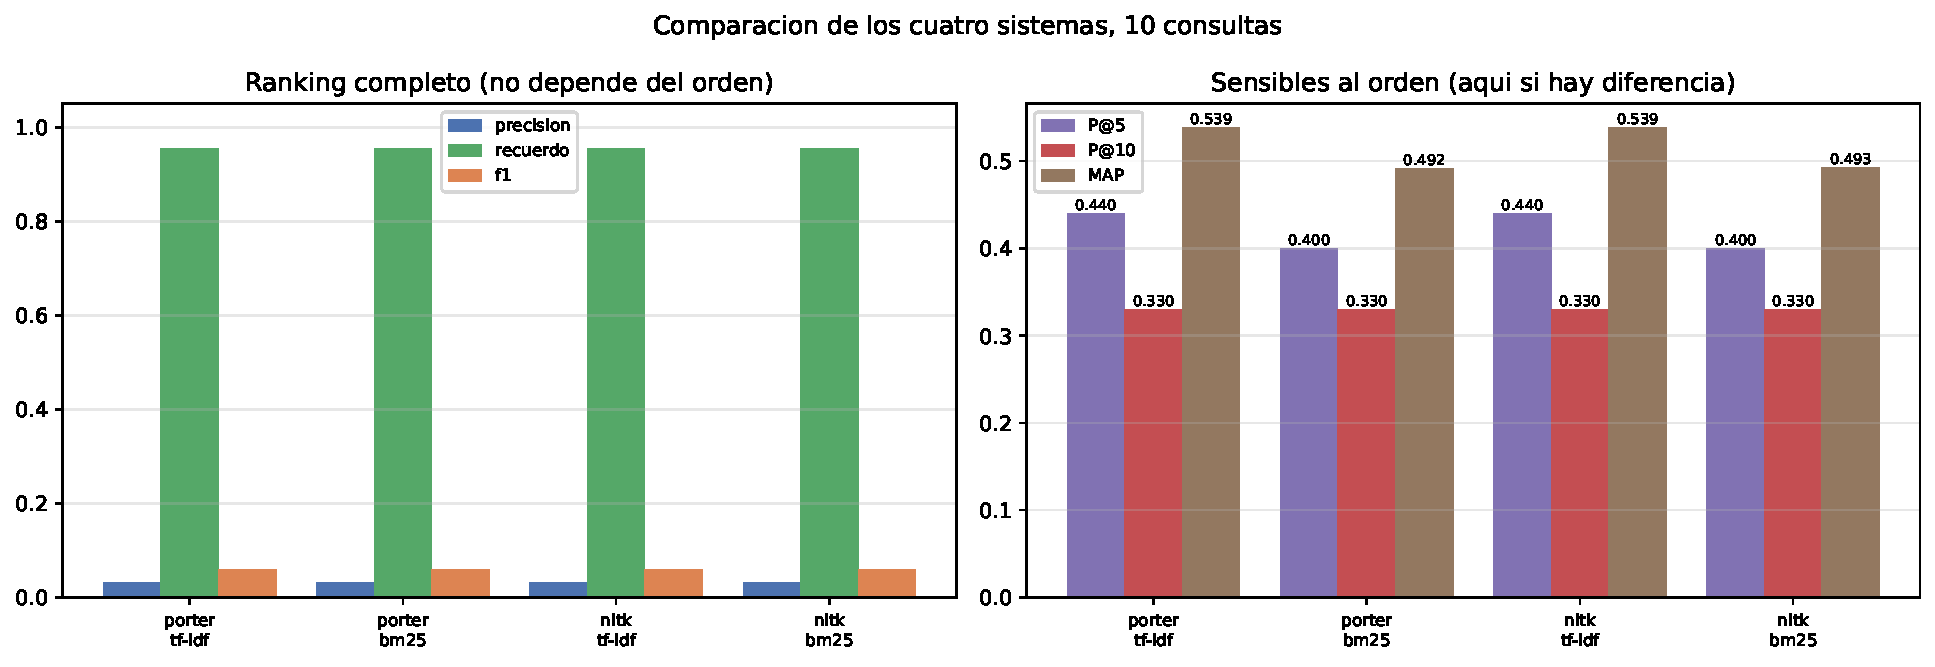
\includegraphics[width=\linewidth]{comparacion_sistemas.pdf}
  \caption{Métricas de los cuatro sistemas. Del lado izquierdo las 
  métricas del ranking completo, del derecho las sensibles al orden}
  \label{fig:comparacion}
\end{figure}

\subsection*{Posición de los documentos relevantes}

\begin{table}[H]
  \centering
  \begin{tabular}{rcllrr}
    \toprule
    \textbf{Q} & \textbf{Hall.} & \textbf{Posiciones tf-idf}
      & \textbf{Posiciones BM25} & \textbf{AP tf-idf}
      & \textbf{AP BM25} \\
    \midrule
     1 & 7/7 & 1, 3, 4, 6, 7, 8, 10 & 2, 5, 6, 7, 8, 9, 12
       & 0.7497 & 0.5495 \\
     2 & 2/2 & 1, 5                 & 3, 5
       & 0.7000 & 0.3667 \\
     3 & 3/4 & 3, 13, 41            & 7, 11, 23
       & 0.1401 & 0.1138 \\
     4 & 5/5 & 7, 68, 83, 220, 296  & 14, 74, 180, 219, 311
       & 0.0487 & 0.0299 \\
     5 & 4/5 & 17, 28, 64, 126      & 12, 19, 57, 129
       & 0.0418 & 0.0544 \\
     6 & 9/9 & 1, 2, 3, 4, 5, 6, 8, 11, 15
             & 1, 2, 3, 4, 5, 6, 8, 9, 13
       & 0.9114 & 0.9396 \\
     7 & 2/2 & 26, 89               & 8, 118
       & 0.0305 & 0.0710 \\
     8 & 2/2 & 1, 2                 & 1, 2
       & 1.0000 & 1.0000 \\
     9 & 8/8 & 1, 2, 3, 4, 5, 6, 7, 23
             & 1, 2, 3, 4, 5, 6, 7, 16
       & 0.9185 & 0.9375 \\
    10 & 6/6 & 1, 2, 3, 5, 8, 9     & 1, 2, 4, 5, 6, 8
       & 0.8486 & 0.8556 \\
    \bottomrule
  \end{tabular}
  \caption{En qué lugar del ranking sale cada documento relevante,
    sobre el corpus de Porter. Hall. es cuántos de los relevantes se
    alcanzaron a recuperar.}
  \label{tab:posiciones}
\end{table}

\begin{table}[H]
  \centering
  \begin{tabular}{rcllrr}
    \toprule
    \textbf{Q} & \textbf{Hall.} & \textbf{Posiciones tf-idf}
      & \textbf{Posiciones BM25} & \textbf{AP tf-idf}
      & \textbf{AP BM25} \\
    \midrule
     1 & 7/7 & 1, 3, 4, 6, 7, 8, 10   & 2, 5, 6, 7, 8, 9, 12
       & 0.7497 & 0.5495 \\
     2 & 2/2 & 1, 5                   & 3, 5
       & 0.7000 & 0.3667 \\
     3 & 3/4 & 3, 13, 41              & 7, 11, 23
       & 0.1401 & 0.1138 \\
     4 & 5/5 & 7, 68, 83, 215, 288    & 14, 75, 173, 220, 306
       & 0.0489 & 0.0300 \\
     5 & 4/5 & 17, 28, 64, 126        & 12, 19, 57, 129
       & 0.0418 & 0.0544 \\
     6 & 9/9 & 1, 2, 3, 4, 5, 6, 8, 11, 15
             & 1, 2, 3, 4, 5, 6, 7, 9, 13
       & 0.9114 & 0.9535 \\
     7 & 2/2 & 26, 89                 & 8, 118
       & 0.0305 & 0.0710 \\
     8 & 2/2 & 1, 2                   & 1, 2
       & 1.0000 & 1.0000 \\
     9 & 8/8 & 1, 2, 3, 4, 5, 6, 7, 23
             & 1, 2, 3, 4, 5, 6, 7, 16
       & 0.9185 & 0.9375 \\
    10 & 6/6 & 1, 2, 3, 5, 8, 9       & 1, 2, 4, 5, 6, 8
       & 0.8486 & 0.8556 \\
    \bottomrule
  \end{tabular}
  \caption{Lo mismo sobre el corpus de NLTK}
  \label{tab:posiciones-nltk}
\end{table}

\section{Discusión}

\subsection*{Por qué los cuatro sistemas empatan en P, R y $F_1$}

Un documento entra al ranking si su coseno es distinto de cero, es
decir si comparte al menos un término con la consulta. Esa condición
no depende del pesado, es decir, los pesos cambian el valor del coseno,
no si es cero o no. Se verificó que el conjunto recuperado es
literalmente el mismo entre tf-idf y BM25 en todas las consultas
probadas, y que entre Porter y NLTK difiere a lo mucho en 4 documentos,
por los términos donde los dos truncadores (Porter y NLTK) discrepan.


\subsection*{tf-idf resulta mejor que BM25}

Según recuerdo, OkapiBM25 se presenta como una mejora o refinamiento de 
tf-idf pero en nuestro experimento, con MAP de $0.5389$ contra $0.4918$ y
 P@5 de $0.44$ contra $0.40$,
tf-idf gana, lo cual es contradictorio. 
Dos razones lo explican. La primera es la saturación:
BM25 aplana las frecuencias altas, y en documentos cortos de revista
que un término aparezca diez veces sí es señal fuerte del tema, así
que aplanarla tira información útil. La segunda es que BM25 está
calibrado para consultas con pesos propios, y aquí las consultas son
binarias (constraints del experimento).

La ventaja no es uniforme. BM25 gana en las consultas 5, 6, 7, 9 y 10,
y pierde por mucho en la 1, la 2 y la 4. En la consulta 2 la
diferencia de AP es de $0.70$ contra $0.37$ por mover un solo
documento de la posición 1 a la 3.

\subsection*{Porter original VS NLTK}

Son prácticamente el mismo sistema; MAP idéntico hasta el cuarto
decimal en tf-idf ($0.5389$) y una diferencia de $0.0014$ en BM25, que
es ruido. Matchea con lo medido en la actividad 1, donde los dos
modos difieren en el $1.73\%$ de los tokens. La elección del modo de
truncamiento no tiene consecuencias prácticas, al menos en esta colección.


\section{Conclusiones}

El sistema funciona. Con el mapeo correcto de los juicios, MAP de
$0.5389$ y P@10 de $0.33$ sobre las primeras 10 consultas, con cuatro
consultas que colocan todos sus relevantes dentro de los primeros
quince resultados.

La lección metodológica principal es que, la métrica tiene que
corresponder a lo que se quiere comparar. Precisión, recuerdo y $F_1$
sobre el ranking completo son incapaces de distinguir un pesado de
otro, no por un defecto del experimento sino porque miden otra cosa.
Reportarlas solas habría llevado a concluir que los cuatro sistemas
son equivalentes, lo cual sería incorrecto.

Igual, queda pendiente extender la evaluación a las 83 consultas. Con solo
diez, una diferencia de MAP de $0.047$ entre tf-idf y BM25 no tiene
respaldo estadístico suficiente para afirmarse como general, así como
probar con pesos propios en las consultas.

\section*{Entregables}

En \texttt{out/actividad\_2/}, una línea por consulta con el formato
\texttt{Q<id> D<id> sim ... P R F1}, con todos los documentos de
coseno distinto de cero en orden decreciente:

\begin{center}
\begin{tabular}{ll}
    \toprule
    \texttt{rec\_porter\_tfidf.txt} & Porter con tf-idf \\
    \texttt{rec\_porter\_bm25.txt}  & Porter con Okapi BM25 \\
    \texttt{rec\_nltk\_tfidf.txt}   & NLTK con tf-idf \\
    \texttt{rec\_nltk\_bm25.txt}    & NLTK con Okapi BM25 \\
    \bottomrule
\end{tabular}
\end{center}

El código está en \texttt{src/actividad.ipynb} y el entorno en
\texttt{../requirements.txt}. Se agregó \texttt{matplotlib} para las
gráficas comparativas.

\section*{Referencias}

\begin{enumerate}[label={[\arabic*]}, itemsep=0.3em, leftmargin=*]
    \item \textbf{Colección Time.} IR Group, University of Glasgow.
          Colecciones de prueba para recuperación de información.\\
          \url{http://ir.dcs.gla.ac.uk/resources/test_collections/}\\
          El archivo \texttt{README} de la colección es el que aclara
          que son 425 documentos con huecos en la numeración.
    \item \textbf{Algoritmo de Porter.} Martin Porter.\\
          \url{https://tartarus.org/martin/PorterStemmer/}\\
          Publicado como \emph{An algorithm for suffix stripping}
    \item \textbf{Okapi BM25.} Robertson y Walker,
          \emph{Some simple effective approximations to the 2-Poisson
          model for probabilistic weighted retrieval}, SIGIR 1994.\\
          \url{https://dl.acm.org/doi/10.5555/188490.188561}
\end{enumerate}

\appendix

\end{document}

%############################ END OF REPORTE_2.TEX #############################
%###############################################################################
